\documentclass[11pt, oneside, reqno]{amsart}
\usepackage{fullpage}
\usepackage{amssymb,latexsym,amsmath,verbatim,layout,hyperref,amsthm,color,graphicx,mdframed,tikz,geometry,inputenc}  
\numberwithin{equation}{section}
\usepackage[T1]{fontenc}
%\usepackage[light,math]{anttor}
\usepackage {mathrsfs}
%package for good looking widehat
\usepackage{hyperref}
\usepackage{cleveref}
\usepackage{scalerel}

\makeatletter
\newcommand\makebig[2]{%
  \@xp\newcommand\@xp*\csname#1\endcsname{\bBigg@{#2}}%
  \@xp\newcommand\@xp*\csname#1l\endcsname{\@xp\mathopen\csname#1\endcsname}%
  \@xp\newcommand\@xp*\csname#1r\endcsname{\@xp\mathclose\csname#1\endcsname}%
}
\makeatother

\makebig{biggg} {3.0}
\makebig{Biggg} {3.5}
\makebig{bigggg}{4.0}
\makebig{Bigggg}{4.5}            
% AMS Theorems  
\theoremstyle{plain}% default
%\newtheorem{name}[counter]{text}[section]
\newtheorem{thm}{Theorem}[section]
\newtheorem{lem}[thm]{Lemma}
\newtheorem{prop}[thm]{Proposition}
\newtheorem{q}{Question}
\newtheorem*{ans}{Answer}
\newtheorem*{cor}{Corollary}


\theoremstyle{definition}
\newtheorem{defn}[thm]{Definition}
\newtheorem{conj}[thm]{Conjecture}
\newtheorem{exmp}[thm]{Example}


\theoremstyle{remark}
\newtheorem*{rmk}{Remark}
\newtheorem*{note}{Note}
\newtheorem{case}{Case}
\newtheorem{ex}{Exercise}
\newtheorem{eg}{Example}
\usepackage{hyperref}
\def\ci{\perp\!\!\!\perp}
\newcommand*{\bigchi}{\mbox{\Large$\chi$}} 
\renewcommand{\vec}[1]{\mathbf{#1}}


\newcommand{\e}{\mathbf{e}} 
    

\newcommand{\vgrad}{\mathbf{\nabla}}     
\newcommand{\vlap}{\mathbf{\Delta}}     
\newcommand{\sph}{\mathbb{S}}
%	x=  x,\quad  u,\quad \vgrad,\quad \vlap,\quad \sph
\newcommand{\R}{\mathbb{R}}
\renewcommand{\P}{\mathbb{P}}
\newcommand{\E}{\mathbb{E}}
\newcommand{\N}{\mathbb{N}}
\newcommand{\F}{\mathbb{F}}
\newcommand{\s}{\mathfrak{s}}
\newcommand{\A}{\mathcal{A}}

%\newcommand{\mbpRectIntensity}{\hat{\xi}^{\sqbullet}}

%geometry
\newcommand{\rectangle}{\tikz \fill [black] (0.1, 0.1) rectangle (0.2,0.2);}
\newcommand{\trapezoid}{\tikz \fill [black] (0.1, 0.2) -- (0.2,0.3) -- (0.3,0.3) -- (0.3,0.2) -- (0.1,0.2);}


\title{Power flow analysis
}


\author{Leanne Dong}

\date{\today}
\begin{document}
	\maketitle

\section{Introduction}
	Power flow analysis is a fundamental study discussed in any power system analysis textbook. The objective is to calculate the voltages (magnotude and angle) for a given load, generation and network condition. Once voltages are known for all buses, line flow and losses can be calculated. The starting point of solving power flow problem is to identify the known and unknown variables in the system. Based on these variables, buses are classified into three types: slack, generation (PV) and load buses (PQ). To recap Khaled's note, the slack bus is required to provide the mimatch between scheduled generation and total system load including losses and total generation. The slack bus is monthly considered as the reference bus because both voltage magnitude and angles are specified. The rest of generator buses are called regulated or PV buses as the net real power is specified and voltage magnitude is regulated. Most of the buses in practical power systems are load buses, the so-called PQ buses, since both net real and reactive power loads are specified.

For PQ buses, boh voltage magnitudes and angles are unknown, whereas for PV buses, only the voltage angle is unknown. As both voltage magnitudes and angles are specified for the Slack bus, there are no variables need to be solved. In a system with $n$ buses and $g$ generators, there are $2(n-1)-(g-1)$ unknowns. To solve these unknowns, real and reactive power balance equations are used. To write these equations, we need to model the transmission network using the admittance matrix ($Y$-bus)
In this note, I will mainly focus on the computation
of Jacobian matrix for Newton Raphson method.

\section{Admittance matrix and power flow equation}
\begin{align}
	A = \begin{bmatrix} 
	    Y_{11} & \dots & Y_{1n} \\
	    \vdots & \ddots & \\
	    a_{n1} & \dots & a_{nn} 
	    \end{bmatrix}
\end{align}
The values of diagonal elements $(Y_{ii})$ are equal to the sum of the admittances connected to bus $i$. The off-diagonal element $(Y_{ij})$ are equal to the negative of the admittance connecting the two buses $i$ and $j$. It is worth noting that with large system, $Y$-bus is a sparse matrix.
   \begin{align}
   	Y_{ii}&=\sum^n_{\substack{j=0 \\ j\neq i}}y_{ij}\label{yii}\\
	Y_{ij}&=Y_{ji}=-y_{ij}\label{yij}
   \end{align}
The net injected power at any bus can be calculated using the bus voltage ($V_i$), neighboring bus voltage $(V_j)$, and the admittances between the bus and its neighboring buses $(y_{ij})$ is
\begin{align*}
	I_i &= V_i y_{i0}+(V_i-V_1)y_{i1}
	+(V_i-V_2)y_{i2}+\cdots+(V_i-V_j)y_{ij}
\end{align*}
Rearranging the elements as function of voltages, the current equation becomes as follows:
\begin{align*}
	I_i&=V_i(y_{i0}+y_{i1}+y_{i2}+\cdots+y_{ij})-V_1 y_{i1} - V_2 y_{i2} - \cdots - V_j y_{ij}
\end{align*}


%\begin{align*}
\[
	I_i=V_i\sum_{\substack{j=0 \\ j\neq i}}y_{ij}-\sum_{\substack{j=1 \\ j\neq i}}y_{ij}= V_i Y_{ii}+\sum_{j=1\\ j\neq i}Y_{ij}V_j
\]
%\end{align*}

The complex power equation at any bus can be written as follows:
\begin{align*}
	S_i=P_i+jQ_1=V_i I^*_i
\end{align*}
or
\begin{align*}
	S^*_i=P_i-jQ_1=V^*_i I_i
\end{align*}
The complex power equation at any bus can be written as follows:
Substitututing the expression on the current in $S^*_i$ equation results in the following formula:

\[
	S^*_i = V^*_i\left(V_i\sum_{\substack{j=0 \\ j\neq i}}y_{ij}-\sum_{\substack{j=1 \\ j\neq i}}y_{ij}\right)
	= V^*_i\left(V_i Y_{ii}+\sum_{j=1\\ j\neq i}Y_{ij}V_j\right)
\]

Real and reactive power can be calculated from the following equations:
\[
	P_i=\text{Re}\Biggggl\{V^*_i\left(V_i\sum_{\substack{j=0 \\ j\neq i}}y_{ij}-\sum_{\substack{j=1 \\ j\neq i}}y_{ij}V_j\right)\Biggggr\}=\text{Re}\Biggggl\{V^*_i\left(V_i Y_{ii}+\sum_{j=1\\ j\neq i}Y_{ij}V_j\right)\Biggggr\}
\]
	      
\[	
Q_i=-\text{Im}\Biggggl\{V^*_i\left(V_i\sum_{\substack{j=0 \\ j\neq i}}y_{ij}-\sum_{\substack{j=1 \\ j\neq i}}y_{ij}V_j\right)\Biggggr\}=-\text{Im}\Biggggl\{V^*_i\left(V_i Y_{ii}+\sum_{j=1\\ j\neq i}Y_{ij}V_j\right)\Biggggr\}
\]
or simply
\begin{align}
	P_i&=\sum^n_{j=1}|V_i||V_j||Y_{ij}|\cos(\theta_{ij}-\delta_i+\delta_j)\label{PV}\\
	Q_i&=-\sum^n_{j=1}|V_i||V_j||Y_{ij}|\sin(\theta_{ij}-\delta_i+\delta_j)\label{PQ}
\end{align}
And the current ($I_i$) can be written as a function of the power as follows:
\[
 \frac{P_i-jQ_i}{V^*_i}=V_i\sum_{\substack{j=0 \\ j\neq i}}y_{ij}-\sum_{\substack{j=1 \\ j\neq i}}y_{ij}V_j = V_i Y_{ii}+\sum_{j=1\\ j\neq i}Y_{ij}V_j
\]
\begin{figure}[!ht]
  \centering
  \begin{minipage}[b]{0.5\textwidth}
    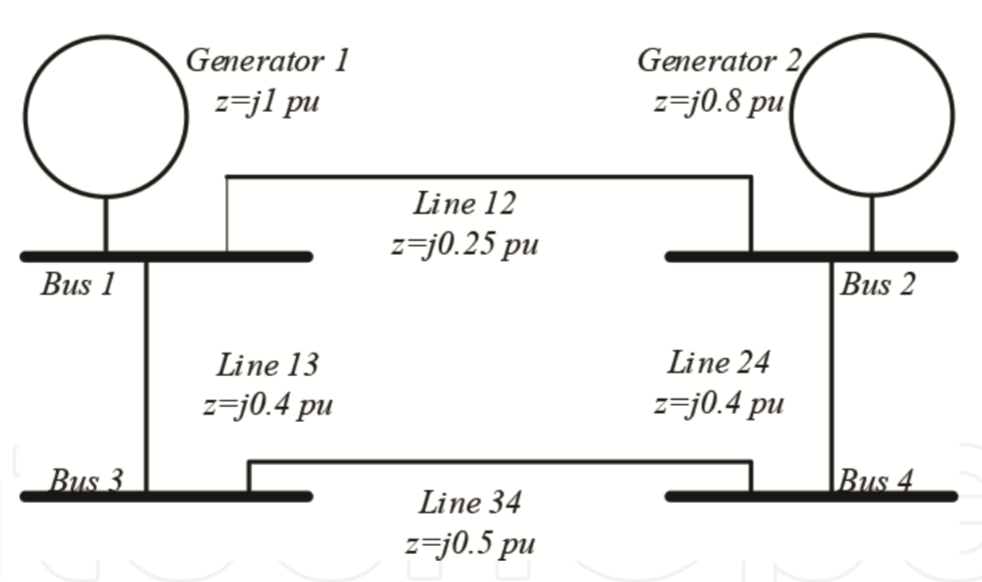
\includegraphics[width=\textwidth]{fig2.png}
    \caption[figure 2]{Impedance diagram}
  \end{minipage}
  \hfill
  \begin{minipage}[b]{0.5\textwidth}
    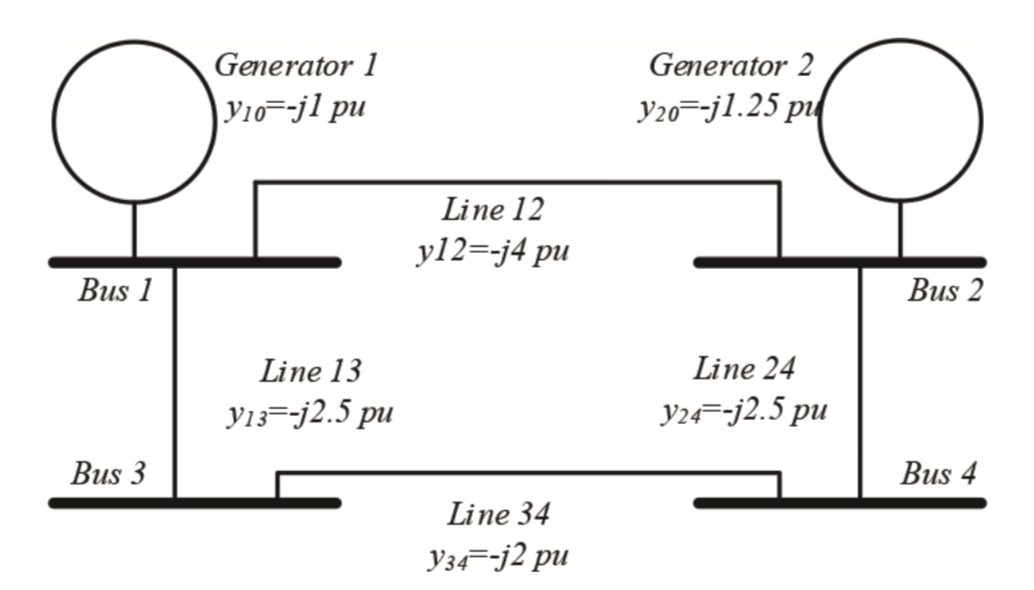
\includegraphics[width=\textwidth]{fig3.png}
    \caption[figure 3]{Admittance diagram}
    \label{fig:eg3}
  \end{minipage}
\end{figure}

\section{Newton-Raphson technique}

The Newton-Raphson (NR) technique, also known as the method of successive approximation, is based on Taylor's expansion approximation. The unknown $x$ in the function $f(x)=c$ can be solved via the Taylor's expansion approximation. Starting with an initial estimate $x^{(0)}$, the estimation error is $\Delta x^{(0)}$. Applying Taylor's expansion approximation, the function can be written as
\begin{align}
	f(x^{(0)}+\Delta x^{(0)})=c
\end{align}
\begin{align}
	f(x^{(0)}+\Delta x^{(0)})=f(x^{(0)})+f'(x^{(0)})\Delta x^{(0)}+\frac{1}{2!}f''(x^{(0)})\Delta x^{(0)^2} +\frac{1}{3!}f^{(3)}(x^{(0)})\Delta x^{(0)^2}+\cdots = c
\end{align}

Assuming $\Delta x^{(0)})$ is small, the higher order terms $\frac{1}{2!}f''(x^{(0)})\Delta x^{(0)^2} +\frac{1}{3!}f^{(3)}(x^{(0)})\Delta x^{(0)^2}+\cdots$ are neglected and the function can be approximated by the first two terms, namely,
\begin{align}
	f(x^{(0)}+\Delta x^{(0)})\approx f(x^{(0)})+f'(x^{(0)})\Delta x^{(0)}=c
\end{align}

Based on $x^{(0)}$, the derivation from the correct solution can be iteratively calculated.
\begin{align}
	\Delta x^{(0)}=\frac{c-f(x^{(0)})}{f'(x^{(0)})}=\frac{\Delta f(x^{(0)})}{f'(x^{(0)})}
\end{align}

The improved solution can be calculated iteratively.
\begin{align}
	x^{(1)}=x^{(0)}+\Delta x^{(0)}
\end{align}
The iterative process is stopped when the mismatch between scheduled and calculated value ($\Delta f^{(k)}=c-f(x^{(k)})$) is within tolerence limit $|\Delta f^{(k)}|\le \epsilon$.
In the context of power flow problems, unknown variables $x$ are both voltage magnitude $|V_i|$ and angles $\angle \delta_i$ at load buses, as well as voltage angle ($\angle \delta_i$) at regulated buses. The scheduled (specified) quantitties $(c)$ are both net real ($P^{sch}_i$) and reactive power $(jQ^{sch}_i)$ values at load buses and real power at generation buses. The iterative values of real power are calculated using (\ref{PV}) and (\ref{PQ}). Similarly, the iterative values of real power are calculated using 

\[
	P^{(k+1)}_i=\text{Re}\Biggggl\{V^{*(k)}_i\left(V^{(k)}_i\sum_{\substack{j=0 \\ j\neq i}}y_{ij}-\sum_{\substack{j=1 \\ j\neq i}}y_{ij}V^{(k\,\,\text{or}\,\,k+1)}_j\right)\Biggggr\}
\]
or
	      
\[	
P^{(k+1)}_i=\sum^n_{j=1}|V_i|^{(k)}|V_j|^{(k\,\,\text{or}\,\,k+1)}|Y_{ij}|\cos(\theta_{ij}-\delta^{(k)}_i+\delta^{(k)}_j)
\]
The Newton-Rapson power flow formulation can be written as
\begin{align*}
	x^{(k)}=
\begin{bmatrix}
\delta^{(k)}_i\\
|V_i|^{(k)}
\end{bmatrix}
,
c=
\begin{bmatrix}
P^{(sch)}_i\\
Q^{(sch)}_i
\end{bmatrix}
,
f=
\begin{bmatrix}
P^{(k)}_i\\
Q^{(k)}_i
\end{bmatrix}
\text{and}
\begin{bmatrix}
P^{(sch)}_i\\
Q^{(sch)}_i
\end{bmatrix}
-
\begin{bmatrix}
P^{(k)}_i\\
Q^{(k)}_i
\end{bmatrix}
=
\begin{bmatrix}
\Delta P^{(k)}_i\\
\Delta Q^{(k)}_i
\end{bmatrix}
\end{align*}


In a multivariable setup, the derivative $f'$ is replaced by partial derivatives with respect to different variables. The Jacobian matrix is represented as
\begin{align}
	f'&=
	\begin{bmatrix}
		\frac{\partial P_i}{\partial\delta_i} & \frac{\partial P_i}{\partial |V_i|}\\
		\frac{\partial Q_i}{\partial\delta_i} & \frac{\partial Q_i}{\partial |V_i|}
	\end{bmatrix}
	= 
	\begin{bmatrix}
		J_{P\delta} & J_{P|V|}\\
		J_{Q\delta} & J_{Q|V|}
	\end{bmatrix}
\end{align}
Therefore, the power flow can be solved using 
\[\begin{bmatrix}
P^{(sch)}_i\\
Q^{(sch)}_i
\end{bmatrix}
-
\begin{bmatrix}
P^{(k)}_i\\
Q^{(k)}_i
\end{bmatrix}
=
\begin{bmatrix}
\Delta P^{(k)}_i\\
\Delta Q^{(k)}_i
\end{bmatrix}
= \begin{bmatrix}
		J^k_{P\delta} & J^k_{P|V|}\\
		J^k_{Q\delta} & J^k_{Q|V|}
	\end{bmatrix}^{-1}
	\begin{bmatrix}
	\Delta \delta^{(k)}_i\\
	\Delta |V_i|^{(k)}
	\end{bmatrix}
\]

Therefore the solution can be obtained from the Jacobian matrix in the following sense,
\begin{align*}
	\begin{bmatrix}
	\Delta \delta^{(k)}_i\\
	\Delta |V_i|^{(k)}
	\end{bmatrix}
	=\begin{bmatrix}
	\Delta \delta^{(k-1)}_i\\
	\Delta |V_i|^{(k-1)}
	\end{bmatrix}
	+\begin{bmatrix}
	\Delta \delta^{(k)}_i\\
	\Delta |V_i|^{(k)}
	\end{bmatrix}
\end{align*}
The iterative process stops when the mismatch between calculated and scheduled quantities is within 
$\begin{bmatrix}
	\Delta \delta^{(k)}_i\\
	\Delta |V_i|^{(k)}
	\end{bmatrix}\leq\epsilon$

\begin{eg}[NR power flow solution]
	Solve the power flow problem shown in the following 3-bus system (\ref{fig:eg5})
	\begin{figure}[!ht]
  \centering
    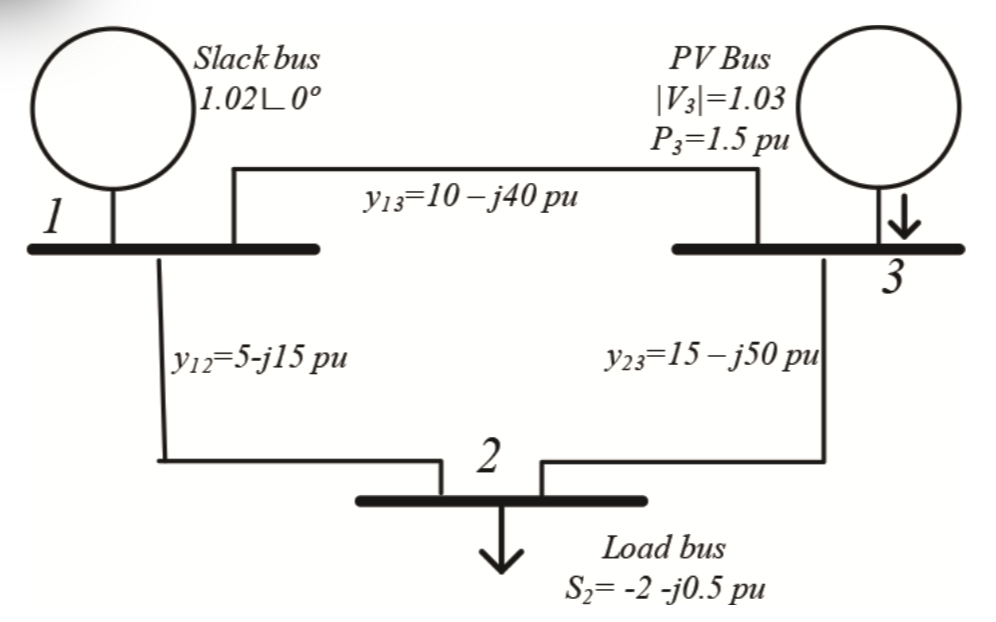
\includegraphics[width=0.5\textwidth]{fig5.png}
    \caption[figure 5]{3-bus power system and flow input data}
    \label{fig:eg5}
    \end{figure}
	 Perform two iterations.
\end{eg}

Solution:

\textit{Step one}: Build Y-bus with equation (\ref{yii}) and (\ref{yij}). So we have
\begin{align*}
	Y&=
	\begin{bmatrix}
		15-j55 & -5+j15 -10+j40\\
		-5+j15 & 20-j65 -15+j50\\
		-10+j40 & -15+j50 25-j90
	\end{bmatrix}
	=
	\begin{bmatrix}
		57.01\angle -74.74^{\circ} & 15.81\angle 108.43^{\circ} & 41.23\angle 104.04^{\circ}\\
		15.81\angle 108.43^{\circ} & 68.01\angle -72.90^{\circ} & 52.20\angle 106.70^{\circ}\\
		41.23\angle 104.04^{\circ} & 52.20\angle 106.70^{\circ} & 93.41\angle -74.48^{\circ}
	\end{bmatrix}
\end{align*}
Since the unknown variables are $\delta_2$, $\delta_3$ and $|V_2|$; the scheduled quantities are 
$P^{sch}_2$, $P^{sch}_3$ and $Q^{sch}_2$, the following problem formulation can be written.

\begin{align*}
	\begin{bmatrix}
		P^{(sch)}_2\\
		P^{(sch)}_3\\
		Q^{(sch)}_2\\
	\end{bmatrix}
	-
	\begin{bmatrix}
		P^{(k)}_2\\
		P^{(k)}_3\\
		Q^{(k)}_2\\
	\end{bmatrix}	
	=
	\begin{bmatrix}
		\frac{\partial P_2^k}{\partial\delta_2} & \frac{\partial P_2^k}{\partial \delta_3} & \frac{\partial P_2^k}{\partial |V_2|}\\
		\frac{\partial P_3^k}{\partial\delta_2} & \frac{\partial P_3^k}{\partial \delta_3} & \frac{\partial P_3^k}{\partial |V_2|}\\
		\frac{\partial Q_2^k}{\partial\delta_2} & \frac{\partial Q_2^k}{\partial \delta_3} & \frac{\partial Q_2^k}{\partial |V_2|}\\
	\end{bmatrix}
	\begin{bmatrix}
		\Delta \delta^{(k)}_2\\
		\Delta \delta^{(k)}_3\\
		\Delta |V_2|^{(k)}
	\end{bmatrix}
\end{align*}

To calculate the Jacobian matrix elements, $P_2$, $P_3$ and $P_3$ equations are obtained using $P_i$ and $Q_i$.

\begin{align*}
	P_2&=\sum^n_{j=1}|V_2||V_j||Y_{2j}|\cos(\theta_{2j}-\delta_2+\delta_j)\\
	&=|V_2||V_1||Y_{21}|\cos(\theta_{21}-\delta_2+\delta_1)+|V_2|^2|Y_{22}|\cos(\theta_{22})+|V_2||V_3||Y_{23}|\cos(\theta_{23}-\delta_2+\delta_3)
\end{align*}

\begin{align*}
	\frac{\partial P_2}{\partial\delta_2}&=|V_2||V_1||Y_{21}|\sin(\theta_{21}-\delta_2+\delta_1)+|V_2||V_3||Y_{23}|\sin(\theta_{23}-\delta_2+\delta_3)
\end{align*}

\begin{align*}
	\frac{\partial P_2}{\partial\delta_3}&=-|V_2||V_3||Y_{23}|\sin(\theta_{23}-\delta_2+\delta_3)
\end{align*}

\begin{align*}
	\frac{\partial P_2}{\partial |V_2|}&=|V_1||Y_{21}|\cos(\theta_{21}-\delta_2+\delta_1)+2|V_2||Y_{22}|\cos(\theta_{22})
+	|V_3||Y_{23}|\sin(\theta_{23}-\delta_2+\delta_3)
\end{align*}

\begin{align*}
	P_3&=\sum^n_{j=1}|V_3||V_j||Y_{3j}|\cos(\theta_{3j}-\delta_2+\delta_j)\\
	&=|V_3||V_1||Y_{31}|\cos(\theta_{31}-\delta_3+\delta_1)+|V_3||V_2||Y_{23}|\cos(\theta_{32}-\delta_3+\delta_2)+|V_3|^2|Y_{33}|\cos(\theta_{33})
\end{align*}

\begin{align*}
	\frac{\partial P_3}{\partial\delta_3}&=|V_3||V_1||Y_{31}|\sin(\theta_{31}-\delta_3+\delta_1)+|V_3||V_2||Y_{32}|\sin(\theta_{32}-\delta_3+\delta_2)
\end{align*}

\begin{align*}
	\frac{\partial P_3}{\partial |V_2|}&=|V_3||Y_{32}|\cos(\theta_{32}-\delta_3+\delta_2)
\end{align*}

\begin{align*}
	Q_2&=-\sum^n_{j=1}|V_2||V_j||Y_{2j}|\sin(\theta_{2j}-\delta_2+\delta_j)\\
	&=-|V_2||V_1||Y_{21}|\cos(\theta_{21}-\delta_2+\delta_1)-|V_2|^2|Y_{22}|\sin(\theta_{22})-|V_2||V_3||Y_{23}|\sin(\theta_{23}-\delta_2+\delta_3)
\end{align*}

\begin{align*}
	\frac{\partial Q_3}{\partial\delta_2}&=|V_2||V_1||Y_{21}|\cos(\theta_{21}-\delta_2+\delta_1)+|V_2||V_3||Y_{23}|\cos(\theta_{23}-\delta_2+\delta_3)
\end{align*}

\begin{align*}
	\frac{\partial Q_3}{\partial\delta_3}&=-|V_2||V_3||Y_{23}|\cos(\theta_{23}-\delta_2+\delta_3)
\end{align*}

\begin{align*}
		\frac{\partial Q_3}{\partial |V_2|}&=-|V_1||Y_{21}|\sin(\theta_{21}-\delta_2+\delta_1)-2|V_2||Y_{22}|\sin(\theta_{22})
-	|V_3||Y_{23}|\sin(\theta_{23}-\delta_2+\delta_3)
\end{align*}
Substitute $|V_1|=1.02$, $|V_3|=1.03$ and $Y_{21}=15.81\angle 108.43^{\circ}$, $\delta_1=0$ to above. And assume that 
\begin{align}
	V^{(0)}_2=1.00\angle 0^{\circ} \quad\text{and}\quad V^{(0)}_3=1.03\angle 0^{\circ}
\end{align}

The calculated quantities: 
\[\begin{bmatrix}
	P^{(1)}_2 \\
	P^{(1)}_3\\
	Q^{(1)}_2
\end{bmatrix} =
\begin{bmatrix}
	-0.5500\\
	0.5665\\
	-1.8000
\end{bmatrix}\]

The scheduled quantities: 
\[\begin{bmatrix}
	P^{(sch)}_2 \\
	P^{(sch)}_3\\
	Q^{(sch)}_2
\end{bmatrix} =
\begin{bmatrix}
	-2\\
	1.5\\
	-0.5
\end{bmatrix}\]

The mismatch power matrix:
\begin{align*}
	\begin{bmatrix}
	\Delta P^{(1)}_2 \\
	\Delta P^{(1)}_3\\
	\Delta Q^{(1)}_2
\end{bmatrix} =
\begin{bmatrix}
	-2\\
	1.5\\
	-0.5
\end{bmatrix}
-
\begin{bmatrix}
	-0.5500\\
	0.5665\\
	-1.8000
\end{bmatrix}
=
\begin{bmatrix}
	-1.45\\
	0.9335\\
	1.3000
\end{bmatrix}
\end{align*}

The Jacobian matrix $J$ elements for the first iteration are 
\begin{align*}
	J&=
	\begin{bmatrix}
	66.8 & -51.5 & 19.45\\
	-51.5 & 93.52 & -15.45\\
	-20.55 & 15.45 & 63.2	
	\end{bmatrix}
\end{align*}

Then continue with the Newton formulation we have

\begin{align*}
	\begin{bmatrix}
		-1.4500\\
		0.9335\\
		1.3000
	\end{bmatrix}
	=
	\begin{bmatrix}
		66.8 & -51.5 & 19.45\\
		-51.5 & 93.52 & -15.45\\
		-20.55 & 15.45 & 63.2
	\end{bmatrix}
	\begin{bmatrix}
		\Delta \delta^{(1)}_2\\
		\Delta \delta^{(1)}_3\\
		\Delta |V_2|^{(1)}
	\end{bmatrix}
\end{align*}
Hence

\begin{align*}
		\begin{bmatrix}
		\Delta \delta^{(1)}_2\\
		\Delta \delta^{(1)}_3\\
		\Delta |V_2|^{(1)}
	\end{bmatrix}
	= 	\begin{bmatrix}
		66.8 & -51.5 & 19.45\\
		-51.5 & 93.52 & -15.45\\
		-20.55 & 15.45 & 63.2
	\end{bmatrix}^{-1}
		\begin{bmatrix}
		-1.4500\\
		0.9335\\
		1.3000
	\end{bmatrix}
	= 
		\begin{bmatrix}
		-0.0279 \text{ rad}\\
		-0.0033 \text{ rad}\\
		0.0123 \text{ pu}
	\end{bmatrix}
\end{align*}

Then 
\begin{align*}
	\begin{bmatrix}
		 \delta^{(1)}_2\\
		 \delta^{(1)}_3\\
		  |V_2|^{(1)}
	\end{bmatrix}
= 	\begin{bmatrix}
		 \delta^{(0)}_2\\
		 \delta^{(0)}_3\\
		  |V_2|^{(0)}
	\end{bmatrix}
+
	\begin{bmatrix}
		\Delta \delta^{(1)}_2\\
		\Delta \delta^{(1)}_3\\
		\Delta |V_2|^{(1)}
	\end{bmatrix}
\end{align*}

Now we move to the second iteration, consider


\begin{align}
	V^{(1)}_2=1.0123\angle -1.5986^{\circ} \quad\text{and}\quad V^{(1)}_3=1.03\angle -0.1891^{\circ}
\end{align}

The calculated quantities: 
\[\begin{bmatrix}
	P^{(2)}_2 \\
	P^{(2)}_3\\
	Q^{(2)}_2
\end{bmatrix} =
\begin{bmatrix}
	-2.0109\\
	1.5202\\
	-0.4621
\end{bmatrix}\]

The mismatch power matrix:
\begin{align*}
	\begin{bmatrix}
	\Delta P^{(2)}_2 \\
	\Delta P^{(2)}_3\\
	\Delta Q^{(2)}_2
\end{bmatrix} =
\begin{bmatrix}
	-2\\
	1.5\\
	-0.5
\end{bmatrix}
-
\begin{bmatrix}
	-2.0109\\
	1.5202\\
	-0.4621
\end{bmatrix}
=
\begin{bmatrix}
	-0.0109\\
	-0.0202\\
	-0.0379
\end{bmatrix}
\end{align*}

The Jacobian matrix $J$ elements for the second iteration are 
\begin{align*}
	J&=
	\begin{bmatrix}
	67.07 & -51.74 & 18.26\\
	-52.50 & 94.49 & -14.18\\
	-22.51 & 16.91 & 65.34	
	\end{bmatrix}
\end{align*}


\begin{align*}
		\begin{bmatrix}
		\Delta \delta^{(2)}_2\\
		\Delta \delta^{(2)}_3\\
		\Delta |V_2|^{(2)}
	\end{bmatrix}
	= 	\begin{bmatrix}
		67.07 & -51.74 & 18.26\\
	-52.50 & 94.49 & -14.18\\
	-22.51 & 16.91 & 65.34	
	\end{bmatrix}^{-1}
		\begin{bmatrix}
		-2.0109\\
		1.5202\\
		-0.4621
	\end{bmatrix}
\end{align*}

Then 
\begin{align*}
	\begin{bmatrix}
		\Delta \delta^{(2)}_2\\
		\Delta \delta^{(2)}_3\\
		\Delta |V_2|^{(2)}
	\end{bmatrix}
= 	
\begin{bmatrix}
	0.1272\times 10^{-3} \text{ rad}\\
	-0.2154\times 10^{-3} \text{ rad}\\
	-0.4810\times 10^{-3} \text{ pu}
\end{bmatrix}
\end{align*}


\begin{align*}
	\begin{bmatrix}
		 \delta^{(2)}_2\\
		 \delta^{(2)}_3\\
		  |V_2|^{(2)}
	\end{bmatrix}
= 	\begin{bmatrix}
		 \delta^{(1)}_2\\
		 \delta^{(1)}_3\\
		  |V_2|^{(1)}
	\end{bmatrix}
+
	\begin{bmatrix}
		\Delta \delta^{(2)}_2\\
		\Delta \delta^{(2)}_3\\
		\Delta |V_2|^{(2)}
	\end{bmatrix}
\end{align*}


\begin{align*}
	\begin{bmatrix}
		 \delta^{(2)}_2\\
		 \delta^{(2)}_3\\
		  |V_2|^{(2)}
	\end{bmatrix}
= 	\begin{bmatrix}
		 -0.0279\quad\text{rad}\\
		 -0.0033\quad\text{rad}\\
		  1.0123\quad\text{pu}
	\end{bmatrix}
+
	\begin{bmatrix}
		 0.1272\times 10^{-3} \text{ rad}\\
	-0.2154\times 10^{-3} \text{ rad}\\
	-0.4810\times 10^{-3} \text{ pu}
	\end{bmatrix}
	= 
\begin{bmatrix}
	-0.0277 \text{ rad}\\
	-0.0035 \text{ rad}\\
	1.0118\text{ pu}
\end{bmatrix}
\end{align*}

It worth noting that the mismatch between the calculated and scheduled quantities diminishes very quickly


\begin{align*}
\begin{bmatrix}
	\Delta P^{(1)}_2 \\
	\Delta P^{(1)}_3\\
	\Delta Q^{(1)}_2
\end{bmatrix}
=
\begin{bmatrix}
	-1.4500\\
	0.9335\\
	1.3000
\end{bmatrix}
\text{and }
\begin{bmatrix}
	\Delta P^{(2)}_2 \\
	\Delta P^{(2)}_3\\
	\Delta Q^{(2)}_2
\end{bmatrix}
=
\begin{bmatrix}
	-0.0109\\
	-0.0202\\
	-0.0379
\end{bmatrix}
\end{align*}

\section{Using graph theory for automated electric circuit solving}
Here we want to implement a computational approach to electric circuit solving based on graph theoretic concepts.

\subsection{Describe the circuit}

\subsection{Find incidence matrix}

\subsection{Finding a set of independent loops}

\subsection{Construction of the spanning tree}

\subsection{Loop oritentation}

\subsection{Circuit equation}

\subsection{Branch currents and voltages}

\subsection{Comparison to SPICE}

\section{Using graph theory for automated thermal-hydraulic network solving}
Our goal here is to solve the thermal network with a few loops in supply and return lines, set up the equation system and solve them. We will implement a multidisciplinary approach combines abstract mathematics, linear algebra, circuit theory and computer programming.

We seek to find the minimum amount of loops that ensure all edges are run through. Particularly, we are concerned with the problem of search and enumeration of all cycles in a graph. And the cycles should include edges. 

From a graph theoretic perspective, we want to find minimal cycles in a graph.
\end{document}